\section{Results using RTL-SDR}

Both the Cumulant method and the Cyclostationary method were rewritten in C++
and placed into a gnuRadio block for use with the RTL-SDR receiver.  Without a
method of generating signals, commonly known signal sources had to be used for
experiementation that were in the frequency range of the receiver.  FM Broadcast
and the BPSK modulated RDS data were the primary signal sets used.

Figure~\ref{fig:SignalOfInterest} shows an averaged Frequency Spectrum from the
RTL-SDR tuned to 88.1Mhz with the sample rate set to 2MSpS.  The FM radio
station at 88.5Mhz is very prevalent and the square signals located to either
side of the signal is either the RDS (Radio Description Service) or the
digital HD Radio data.  

\begin{figure}
\centering
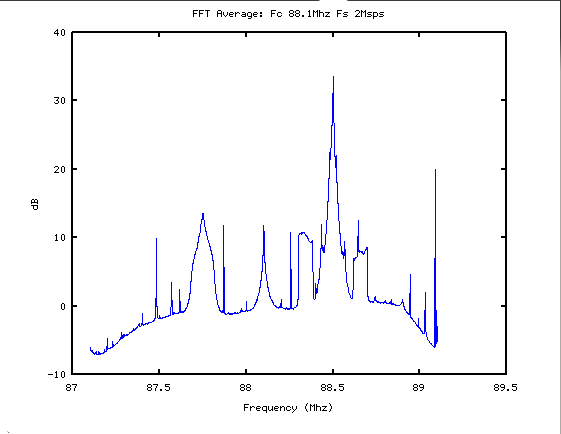
\includegraphics[width=\linewidth]{../img/Report_RTL_SDR_FFT_881M_2Msps.png}
\caption{Spectrum of FM Radio Station located at 88.5 Mhz}
\label{fig:SignalOfInterest}
\end{figure}


\subsection{Cumulant Results}

Time domain classification of unknown signals presents multiple problems
for the implementor.  In simulations, the exact frequency, phase, symbol rate,
and matched filter of the signal is known.  Without this prior knowledge, or the
means of detecting it, blind modulation detection from the time domain becomes a
difficult task.
 
Prior to using the cumulant method to classify the signal, the data was
frequency shifted, filtered, and decimated.  Since no phase lock loop was used,
it is expected that the frequency of the signal of interest will be slightly
different than the tuned frequency.  This will result in a continually rotating
IQ plane.
Earlier we stated that the Cumulant method was phase invarient however this only
applies to a static phase shift and not a continuous rotation.  Without a phase
lock loop, the IQ plane of FM, BPSK, and QAM will be indistinguishable and
resemble a circle with added noise.
AM, SSB-AM, and higher order QAM signals which would not form a single circle in
the IQ domain may still be able to be identified but signal sources of this type
within the frquency range of the RTL-SDR are difficult to find.
Figure~\ref{fig:digitalSignal} shows the spectrum of the digital signal to the
left of the FM station.  This signal was tuned, filtered, and decimated to
isolate the digital signal.  The IQ plot of this data, shown in
Figure~\ref{fig:digitalIQ}, does not provide any information about its content
since, as expected, the symbol rate, exact frequency, are needed.  The Cumulant
method fails to classify the signal correctly and instead classifies it as an AM
signal with $C40 = 0.07$ and $C42 = 0.535$.
Despite the clearer IQ plot, shown in Figure~\ref{fig:FMIQ}, the FM signal is
also missclassified as AM with $C40 = 0.021$ and $C42 =  0.535$.


\begin{figure}
\centering
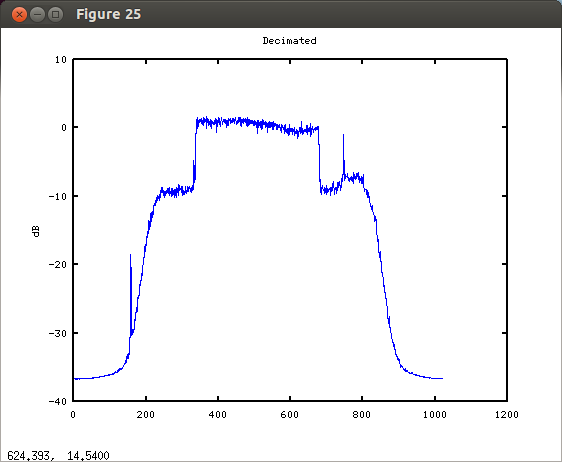
\includegraphics[width=\linewidth]{../img/Report_Decimated_Digital_Signal.png}
\caption{Spectrum of the Digital signal found at 88.34Mhz}
\label{fig:digitalSignal}
\end{figure}

\begin{figure}
\centering
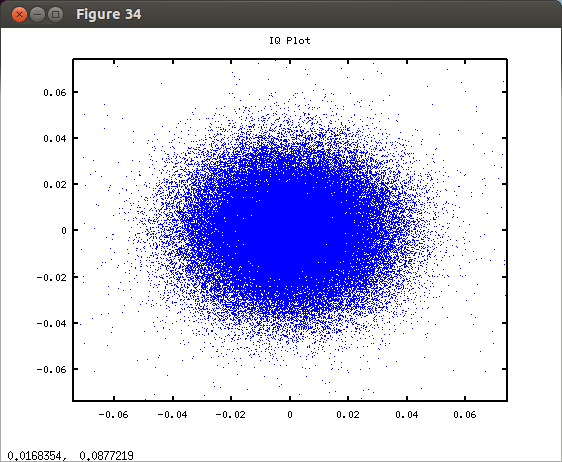
\includegraphics[width=\linewidth]{../img/Report_IQ_Plot_Digital.png}
\caption{IQ Plot of the Digital signal found at 88.34Mhz}
\label{fig:digitalIQ}
\end{figure}

\begin{figure}
\centering
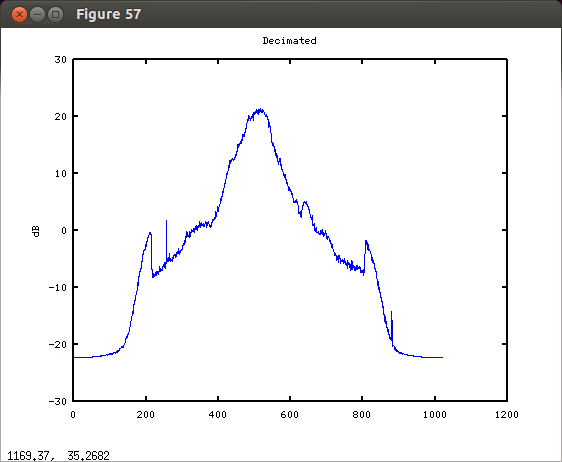
\includegraphics[width=\linewidth]{../img/Report_Decimated_FM_Signal.png}
\caption{Spectrum of the Digital signal found at 88.5Mhz}
\label{fig:FMSignal}
\end{figure}

\begin{figure}
\centering
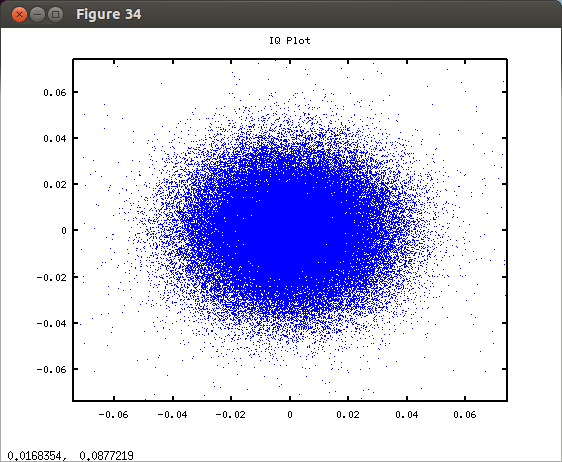
\includegraphics[width=\linewidth]{../img/Report_IQ_Plot_Digital.png}
\caption{IQ Plot of the FM signal found at 88.5Mhz}
\label{fig:FMIQ}
\end{figure}

\subsection{Cyclostationary Results}

The cyclostationary approach discussed in Section~\ref{sec:cycloIntro} depended
on a known template for pattern matching the cycle frequency domain profile. 
This CDP is directly linked to the shape of the frequency domain plot of the
signal.  In real world applications, this shape is based off of factors
including the matched filter used and symbol rate for digital signals and the
frequency deviation and input for FM data.
Modulation classification using the previous made templates is not expected to
do well.  Not only will the unknown variables cause issue but the templates
assumed the signal was the only signal present which is not the case in real
world signals.  Filtering out the other signals would greatly reduce the noise
floor compared to the noisefloor of the template causing additional issues.

Rather than use the cyclostationary detection methods for identification of a
particular modulation based on the previous templates, new templates can be
generated using a known signal and the cyclostationary method can be used to
identify similar signals throughout the spectrum.  The signal was centered at
88.5Mhz, filtered to 600khz and downsampled by a factor of four.
Figure~\ref{fig:decimatedFMandDig} shows the resulting signal. 
Figure~\ref{fig:cycleSpec885} shows the Cycle Spectral Correlation for the
signal, and Figure~\ref{fig:cdp885} shows the cycle domain profile.

\begin{figure}
\centering
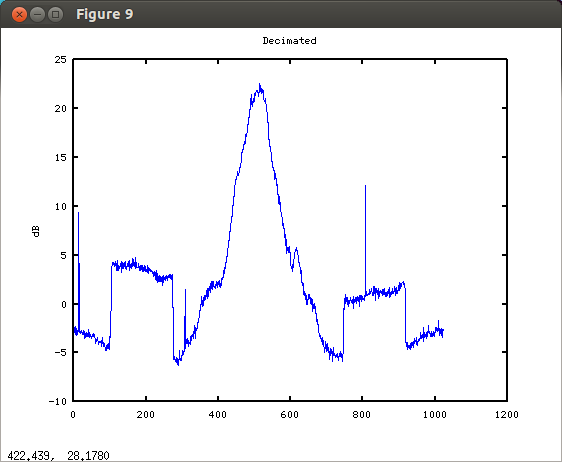
\includegraphics[width=\linewidth]{../img/Report_Decimated_FM_and_Digital.png}
\caption{Decimated FM signal}
\label{fig:decimatedFMandDig}
\begin{comment}
[Sxa Ia] = detectWithRTL_Cyclo(88500000, 4, 600000);
\end{comment}
\end{figure}

\begin{figure}
\centering
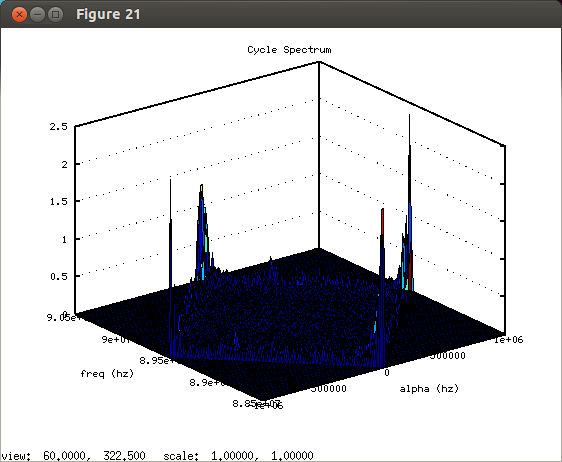
\includegraphics[width=\linewidth]{../img/Report_Cycle_Spectral_Corr_88_5}
\caption{Cycle Spectral Correlation for 88.5Mhz}
\label{fig:cycleSpec885}
\begin{comment}
[Sxa Ia] = detectWithRTL_Cyclo(88500000, 4, 600000);
\end{comment} 
\end{figure}

\begin{figure}
\centering
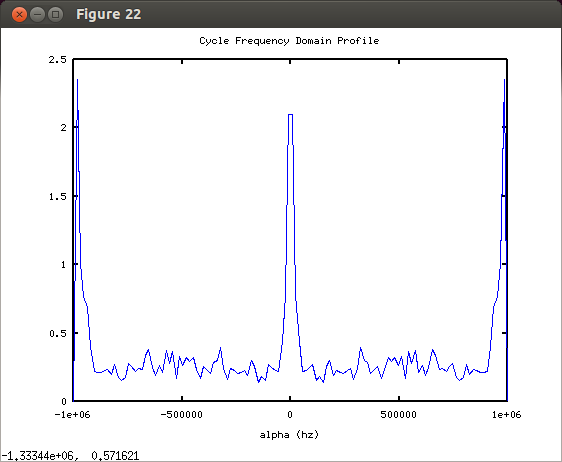
\includegraphics[width=\linewidth]{../img/Report_CDP_885.png}
\caption{CDP for 88.5Mhz}
\label{fig:cdp885}
\begin{comment}
[Sxa Ia] = detectWithRTL_Cyclo(88500000, 4, 600000);
\end{comment}
\end{figure}
